\documentclass[12pt]{beamer}

\usetheme{Malmoe}
\usepackage[utf8]{inputenc}
\usepackage{graphicx}
\usepackage{xcolor}
\usepackage{wrapfig} % texlive-latex-extra package
\usepackage{underscore}
\usepackage{listings}

\definecolor{Cyan}{RGB}{0,141,184}
\definecolor{codeblock}{RGB}{220,220,220}

\setbeamercolor{structure}{fg=Cyan}

\setbeamerfont{title}{series=\bfseries,parent=structure}
\setbeamerfont{subtitle}{size=\normalsize,series=\bfseries,parent=structure}
\setbeamerfont{author}{size=\scriptsize,series=\bfseries,parent=structure}
\setbeamerfont{institute}{size=\scriptsize,series=\bfseries,parent=structure}
\setbeamerfont{date}{size=\scriptsize,series=\bfseries,parent=structure}

%\ shell code block style (https://en.wikibooks.org/wiki/LaTeX/Source_Code_Listings)
\lstset{language=sh,
	basicstyle=\ttfamily\scriptsize,
	backgroundcolor=\color{codeblock},
	commentstyle=\color{blue},
	breaklines=true,
	breakatwhitespace=true,
	showstringspaces=false
}

\title{GIS.lab}
\subtitle{news from development of technology for rapid deployment of complete geospatial infrastructure with supercow capabilities}
\author{Ivan Minčík (imincik)}
%\setbeamercovered{transparent} 
%\setbeamertemplate{navigation symbols}{} 
%\logo{} 
\institute{FOSS4G Europe 2015, Como, Italy}
\date{} 
%\subject{}


% document BEGIN
\begin{document}


\begin{frame}
	\titlepage
\end{frame}

\begin{frame}{The Super Cow}
	\begin{center}
		
\includegraphics[keepaspectratio=true,height=0.6\textheight]{images/cow.png}
	\end{center}
\end{frame}


\section{Introduction}
\begin{frame}
	\begin{center}
		\LARGE\textbf{Introduction}	
	\end{center}
\end{frame}

\begin{frame}{The Problem}
	\begin{center}
		We always \textbf{need more than only one app} for our GIS work flow
	\end{center}
\end{frame}

\begin{frame}{The Problem}
	\begin{center}
		Deployment and maintenance of \textbf{complex system is hard} even if things are going flawlessly
		\end{center}
\end{frame}

\begin{frame}{The Problem}
	\begin{center}
		which usually they are \textbf{not} (:
	\end{center}
\end{frame}

\begin{frame}{GIS.lab}
	\textbf{Instantly} in production with \textbf{no feeding} !
	\begin{center}
		%\ image: cow with QGIS, GRASS and PostGIS in bottles
		
\includegraphics[keepaspectratio=true,height=0.6\textheight]{images/cow.png}
	\end{center}
\end{frame}


\section{What is GIS.lab ?}
\begin{frame}
	\begin{center}
		\LARGE\textbf{What is GIS.lab ?}
	\end{center}
\end{frame}

\begin{frame}{What is GIS.lab ?}
	\textbf{free} technology which can \textbf{instantly} turn pile of metal scrap in to the \textbf{high-end geospatial cluster}
	\begin{center}
		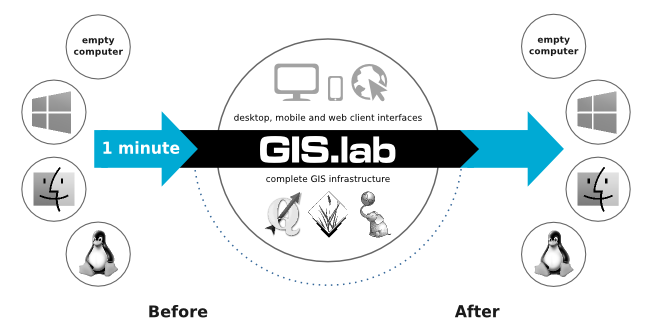
\includegraphics[keepaspectratio=true,height=0.5\textheight]{images/gislab-schema.png}
	\end{center}
\end{frame}

\begin{frame}{What is GIS.lab ?}
	\begin{center}
		and back to \textbf{the same scrap} again
	\end{center}
\end{frame}

\begin{frame}{Features}
	\begin{itemize}[<+->]
		\item so simple \textbf{plug-and-play} deployment as home router
		\item \textbf{central management}
		\item \textbf{desktop, web and mobile} client interfaces
		\item automatic \textbf{clustering and resources sharing}
		\item collaboration tools
		\item fits in your pocket \textbf{pocket}
		\item or \textbf{LAN, data center} and \textbf{cloud}
		\item self contained - no dependency on other service or Internet
	\end{itemize}
\end{frame}

\begin{frame}{GIS.lab Architecture}
	\begin{center}
		%\ image: schema server and clients
		
\includegraphics[keepaspectratio=true,height=0.5\textheight]{images/image.png}
	\end{center}
\end{frame}

\begin{frame}{GIS.lab Server}
	\begin{center}
		%\ image: schema storage and management (gears)
		
\includegraphics[keepaspectratio=true,height=0.5\textheight]{images/image.png}
	\end{center}
	\begin{itemize}
		\item GIS.lab infrastructure orchestration conductor
		\item data storage and sharing
		\item OWS load balancing
		\item central management
		\item client launch support
	\end{itemize}
\end{frame}

\begin{frame}{GIS.lab Clients}
	\begin{center}
		%\image: desktop + web + mobile
		
\includegraphics[keepaspectratio=true,height=0.5\textheight]{images/image.png}
	\end{center}
	\begin{itemize}
		\item launched from GIS.lab Server 
		\item user interfaces for data processing, analysis and collaboration
		\item computing power for GIS.lab Cluster
	\end{itemize}
\end{frame}


\section{What is new ?}
\begin{frame}
	\begin{center}
		\LARGE\textbf{So, what's new ?}	
	\end{center}
\end{frame}

\begin{frame}
	\begin{center}
		mostly \textbf{everything}
	\end{center}
\end{frame}


\section{Deployment}
\begin{frame}
	\begin{center}
		\LARGE\textbf{Deployment}	
	\end{center}
\end{frame}

\begin{frame}{Ansible}
	\begin{center}
		
\includegraphics[keepaspectratio=true,height=0.4\textheight]{images/ansible.png}
	\end{center}
	\begin{itemize}
		\item no requirements on target machine except SSH
		\item idempotent modules, templates
		\item cloud providers AWS, GCE, Digital Ocean, Azure ...
	\end{itemize}
\end{frame}

\begin{frame}[fragile]{Ansible provisioning}
	\begin{center}
		
\includegraphics[keepaspectratio=true,height=0.4\textheight]{images/ansible.png}
	\end{center}

   \lstset{language=sh}
	\begin{lstlisting}
		$ ansible-playbook
		  --inventory=gislab.inventory
		  --private-key=~/.ssh/id_rsa
		  system/gislab.yml
	\end{lstlisting}
\end{frame}

\begin{frame}[fragile]{Virtual Machine - Development and Testing}
	\begin{center}
		
\includegraphics[keepaspectratio=true,height=0.4\textheight]{images/vagrant.png}
		
\includegraphics[keepaspectratio=true,height=0.4\textheight]{images/virtualbox.png}
		
\includegraphics[keepaspectratio=true,height=0.4\textheight]{images/ansible.png}
	\end{center}

   \lstset{language=sh}
	\begin{lstlisting}
		$ vagrant up
		Bringing machine 'gislab_vagrant' up with 'virtualbox' provider...
		==> gislab_vagrant: Importing base box 'precise-canonical'...
		==> gislab_vagrant: Running provisioner: install (ansible)...
	\end{lstlisting}
\end{frame}

\begin{frame}{GIS.lab Unit - End User Deployment}
	\begin{center}
		
\includegraphics[keepaspectratio=true,height=0.5\textheight]{images/gislab-unit.png}
	\end{center}
	\begin{itemize}
		\item portable, pocket size
		\item plug-and-play
		\item automatic adaptation to host network
	\end{itemize}
\end{frame}


\section{Client Interfaces}
\begin{frame}
	\begin{center}
		\LARGE\textbf{Desktop Client}	
	\end{center}
\end{frame}

\begin{frame}{Machines Launch}
	\begin{center}
		%\ image: boot from server - physical client and virtual one
		
\includegraphics[keepaspectratio=true,height=0.5\textheight]{images/image.png}
	\end{center}
	\begin{itemize}
		\item network launch (PXE, HTTP)
		\item physical hardware or virtual client mode
		\item working with every network configuration
	\end{itemize}
\end{frame}

\begin{frame}{Physical or Virtual Mode}
	\begin{center}
		%\ image: Physycal or Virtual Mode
		
\includegraphics[keepaspectratio=true,height=0.5\textheight]{images/image.png}
	\end{center}
	\begin{itemize}
		\item physical mode: best performance, access to original OS is temporary lost
		\item virtual mode: running inside any OS, benefit of using original OS and GIS.lab at once
	\end{itemize}
\end{frame}

\begin{frame}{Desktop Client}
	\begin{center}
		%\ image: desktop client screenshot with QGIS, GRASS ...
		
\includegraphics[keepaspectratio=true,height=0.5\textheight]{images/image.png}
	\end{center}
	\begin{itemize}
		\item QGIS as the geospatial project IDE
		\item integrated with GRASS 7 and others
	\end{itemize}
\end{frame}

\begin{frame}{Maps Publishing on Web}
	\begin{center}
		%\ image: gis.lab web plugin
		
\includegraphics[keepaspectratio=true,height=0.5\textheight]{images/image.png}
	\end{center}
	\begin{itemize}
		\item publish any QGIS project with GIS.lab Web QGIS
	\end{itemize}
\end{frame}

\begin{frame}[fragile]{Customization}
	%\ own client image build system (replacing LTSP)
	\begin{itemize}
		\item customization in isolated environment using standard tools
		\item central image distribution
		\item rollback
	\end{itemize}
	
	\lstset{language=sh}
	\begin{lstlisting}
		$ cp /opt/gislab/client-desktop                  # backup
		     /mnt/backup/client-desktop.backup
		
		$ gislab-client-shell -i   # enter client env
		$ apt-get install gedit    # install Gedit
		$ exit                     # exit client env
		$ gislab-client-image      # deploy updated client image
		
		$ rm -rf /opt/gislab/client-desktop
		  &&
		  mv /mnt/backup/client-desktop.backup
		     /opt/gislab/client-desktop                  # rollback
	\end{lstlisting}
\end{frame}

\begin{frame}{Office Suite}
	\begin{center}
		%\ image: office suite
		
\includegraphics[keepaspectratio=true,height=0.5\textheight]{images/image.png}
	\end{center}
	\begin{itemize}
		\item general usage desktop productivity platform
		\item data storage and sharing
		\item collaboration
		\item central management
	\end{itemize}
\end{frame}


\begin{frame}
	\begin{center}
		\LARGE\textbf{Web and Mobile Client}	
	\end{center}
\end{frame}

\begin{frame}{Web and Mobile Client}
	\begin{center}
		%\ image: web and mobile client screenshots
		
\includegraphics[keepaspectratio=true,height=0.5\textheight]{images/image.png}
	\end{center}
	\begin{itemize}
		\item themes, base and overlay layers
		\item advanced search forms
		\item print outputs
		\item vector features drawing and sharing
	\end{itemize}
\end{frame}


\section{Cluster}
\begin{frame}
	\begin{center}
		\LARGE\textbf{Cluster}	
	\end{center}
\end{frame}

\begin{frame}{Automatic Cluster Orchestration}
	\begin{center}
		
\includegraphics[keepaspectratio=true,height=0.5\textheight]{images/serf.png}
	\end{center}
	\begin{itemize}
		\item server + client machines
		\item decentralized cluster membership and failure detection system based on GOSSIP protocol
	\end{itemize}
\end{frame}

\begin{frame}[fragile]{Cluster Management}
	\textbf{Machines information}

	\lstset{language=sh}
	\begin{lstlisting}
		$ gislab-cluster members

		server.gis.lab  192.168.15.5:7946 
		                alive  role=server

		c50             192.168.15.50:7946
		                alive
		                role=client,worker=yes,session-active=user1

		c51             192.168.15.51:7946
		                left
		                role=client,worker=yes
	\end{lstlisting}
\end{frame}

\begin{frame}[fragile]{Cluster Management}
	\textbf{Events and queries}

	\lstset{language=sh}
	\begin{lstlisting}
		$ gislab-cluster event <EVENT-NAME>
		$ gislab-cluster query <QUERY-NAME>		
	\end{lstlisting}

	\lstset{language=sh}
	\begin{lstlisting}
		$ gislab-cluster event reboot
	\end{lstlisting}
\end{frame}

\begin{frame}[fragile]{Cluster Management}
	\textbf{Executing cross-cluster commands}

	\lstset{language=sh}
	\begin{lstlisting}
		$ MACHINES="$(
		    gislab-cluster members -tag role=client -status=alive
		    | awk -F " " '{printf "%s ", $1}'
		  )"

		$ parallel-ssh
		  -O StrictHostKeyChecking=no -i -H "$MACHINES"

		  sudo DEBIAN_FRONTEND=noninteractive
		  apt-get install -y --no-install-recommends gedit
		  ...
		  [1] 23:02:57 [SUCCESS] c51
		  [1] 23:02:57 [SUCCESS] c51
		  ...
	\end{lstlisting}
\end{frame}

\begin{frame}{Stronger With Each Client Machine}
	\textbf{Universal usage of each machine - full hardware potential utilization}
	\begin{itemize}
		\item desktop working environment
		\item cluster worker node (OWS services, parallel tasks)
	\end{itemize}
\end{frame}

\begin{frame}[fragile]{Stronger With Each Client Machine}
	\textbf{OWS load balancing}

	\lstset{language=sh}
	\begin{lstlisting}
		$ while true; do
		    curl "http://ms.gis.lab:90/cgi-bin/qgis_mapserv?
		      SERVICE=WMS&REQUEST=GetCapabilities"
		  done
	\end{lstlisting}
	\begin{center}
		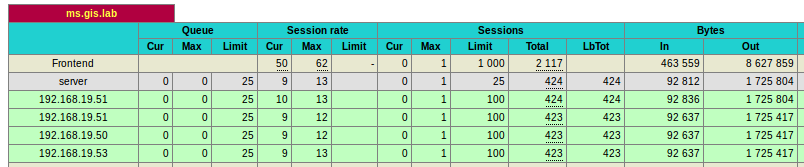
\includegraphics[keepaspectratio=true,width=\textwidth]{images/haproxy-stats.png}
	\end{center}
\end{frame}


\section{Other}
\begin{frame}
	\begin{center}
		\LARGE\textbf{Other}
	\end{center}
\end{frame}

\begin{frame}[fragile]{Tests}
	\textbf{Integration test suite based on Ansible tasks}
	
	\lstset{language=sh}
	\begin{lstlisting}
		$ vagrant provision --provision-with test
		...
		TASK: [basic-server-configuration-test | Test if ordinary test user account exists in PostgreSQL]
		...
		TASK: [service-dns-test | Test 'gis.lab' DNS records are resolved]
		...
		TASK: [service-mapserver-test | Test WMS GetCapabilies request with example GIS.lab project]
		...
		TASK: [service-mapserver-test | Test WMS GetMap request with example GIS.lab project]
		...
	\end{lstlisting}
\end{frame}

\begin{frame}{Where to use ?}
	\begin{itemize}
		\item schools, universities - central management, maintenance-free desktop clients
		\item ...
	\end{itemize}
\end{frame}

\begin{frame}{Future plans}
	\begin{itemize}
		\item integration of WPS services
		\item better integration of GRASS
		\item web administration interface
		\item AWS provider rewrite
		\item web client rewrite with OL 3
		\item update to Ubuntu 16.04 and systemd
	\end{itemize}
\end{frame}

\begin{frame}{Authors}
\end{frame}


% document END
\end{document}